%%%%%%%%%%%%%%%%%%%%%%%%%%%%%%%%%%%%%%%%%
% Beamer Presentation
% LaTeX Template
% Version 1.0 (10/11/12)
%
% This template has been downloaded from:
% http://www.LaTeXTemplates.com
%
% License:
% CC BY-NC-SA 3.0 (http://creativecommons.org/licenses/by-nc-sa/3.0/)
%
%%%%%%%%%%%%%%%%%%%%%%%%%%%%%%%%%%%%%%%%%

%----------------------------------------------------------------------------------------
%	PACKAGES AND THEMES
%----------------------------------------------------------------------------------------

\documentclass{beamer}

\mode<presentation> {

% The Beamer class comes with a number of default slide themes
% which change the colors and layouts of slides. Below this is a list
% of all the themes, uncomment each in turn to see what they look like.

%\usetheme{default}
%\usetheme{AnnArbor}
%\usetheme{Antibes}
%\usetheme{Bergen}
%\usetheme{Berkeley}
%\usetheme{Berlin}
%\usetheme{Boadilla}
%\usetheme{CambridgeUS}
%\usetheme{Copenhagen}
%\usetheme{Darmstadt}
%\usetheme{Dresden}
%\usetheme{Frankfurt}
%\usetheme{Goettingen}
%\usetheme{Hannover}
%\usetheme{Ilmenau}
%\usetheme{JuanLesPins}
%\usetheme{Luebeck}
%\usetheme{Madrid}
%\usetheme{Malmoe}
%\usetheme{Marburg}
%\usetheme{Montpellier}
\usetheme{PaloAlto}
%\usetheme{Pittsburgh}
%\usetheme{Rochester}
%\usetheme{Singapore}
%\usetheme{Szeged}
%\usetheme{Warsaw}

% As well as themes, the Beamer class has a number of color themes
% for any slide theme. Uncomment each of these in turn to see how it
% changes the colors of your current slide theme.

%\usecolortheme{albatross}
%\usecolortheme{beaver}
%\usecolortheme{beetle}
%\usecolortheme{crane}
%\usecolortheme{dolphin}
%\usecolortheme{dove}
%\usecolortheme{fly}
%\usecolortheme{lily}
%\usecolortheme{orchid}
%\usecolortheme{rose}
%\usecolortheme{seagull}
%\usecolortheme{seahorse}
%\usecolortheme{whale}
%\usecolortheme{wolverine}

%\setbeamertemplate{footline} % To remove the footer line in all slides uncomment this line
%\setbeamertemplate{footline}[page number] % To replace the footer line in all slides with a simple slide count uncomment this line

%\setbeamertemplate{navigation symbols}{} % To remove the navigation symbols from the bottom of all slides uncomment this line
}

\usepackage{graphicx} % Allows including images
\usepackage{booktabs} % Allows the use of \toprule, \midrule and \bottomrule in tables
\usepackage{algpseudocode}
\usepackage{verbatim}
\renewcommand{\algorithmicrequire}{\textbf{Input:}} \renewcommand{\algorithmicensure}{\textbf{Output:}}

%----------------------------------------------------------------------------------------
%	TITLE PAGE
%----------------------------------------------------------------------------------------

\title[Gradient Descent Optimization Technics. An overview]{Gradient Descent Optimization Techniques. An overview} % The short title appears at the bottom of every slide, the full title is only on the title page

\author{David Panou} % Your name
\institute[Pierre \& Marie Curie University] % Your institution as it will appear on the bottom of every slide, may be shorthand to save space
{
Pierre \& Marie Curie University \\ % Your institution for the title page
\medskip
\textit{david.panou@gmail.com} % Your email address
}
\date{\today} % Date, can be changed to a custom date

\begin{document}

\begin{frame}
\titlepage % Print the title page as the first slide
\end{frame}

\begin{frame}
\frametitle{Overview} % Table of contents slide, comment this block out to remove it
\tableofcontents % Throughout your presentation, if you choose to use \section{} and \subsection{} commands, these will automatically be printed on this slide as an overview of your presentation
\end{frame}


%----------------------------------------------------------------------------------------
%	PRESENTATION SLIDES
%----------------------------------------------------------------------------------------


%------------------------------------------------
\AtBeginSection[]
  {
     \begin{frame}<beamer>
     \frametitle{Plan}
     \tableofcontents[currentsection]
     \end{frame}
  }
  

\section{Introduction} % Sections can be created in order to organize your presentation into discrete blocks, all sections and subsections are automatically printed in the table of contents as an overview of the talk
%------------------------------------------------

%----------------------------------------------------------------------------------------
%	INTRODUCTION
%----------------------------------------------------------------------------------------

\begin{frame}
\frametitle{Introduction}
This slide is a summary of \cite{Ruder} that introduces optimization techniques for Gradient Descent parameter optimization techniques.\\~\\
We will go through the most commonly used and implemented Gradient Descent Strategies and give intuitive idea behind there formalization.

\end{frame}

%------------------------------------------------

\section{Standard Gradient Descent Techniques} % Sections can be created in order to organize your presentation into discrete blocks, all sections and subsections are automatically printed in the table of contents as an overview of the talk
%------------------------------------------------

\begin{frame}
\frametitle{Introduction}
Before jumping into Gradient Descent strategy, we would like to remind to the reader the different existing Gradient Descent Formalization.\\~\\
Those methods are dealing with the way the trained dataset is presented to the network
As simple method, they doesn't adapt themselves to the problem at hand as each parameter (i.e learning rate, stopping) have to be set by hand

\end{frame}


\subsection{Stochastic Gradient Formalization}
\begin{frame}
\frametitle{Gradient Descent Formalization}

\begin{block}{Definition}

Gradient Descent procedures takes a learning problem and try to find a solution of set of linear inequalities \\~\\
It does so by defining a criterion function $J(\theta)$, that is minimized if $ \theta^T y_{i} > 0$, with $\theta$ being the algorithm parameters.\\~\\
This very simple procedure reduces the learning problem to minimizing a scalar function.
\end{block}
The gradient descent pseudo algorithm is given at the end of those slide as a reminder.
\end{frame}

\subsection{Batch Gradient Descent}
\begin{frame}
\frametitle{Batch Gradient Descent}

\begin{block}{Definition}
The most simple formalization of Gradient Descent is the Batch Gradient Descent.
In Batch Gradient Descent, the learning algorithm takes all of the training dataset points at each training epoch.
\end{block}

\begin{block}{Characteristics}
Batch gradient descent is guaranteed to converge to the global minimum for convex functions and to a local minimum for non-convex ones.\\~\\

However it can be intractable for datasets that doesn't fit in memory and can be very slow. Finally, for large datasets it performs redundant computations. Those problems are addressed by Stochastic Gradient Descent.
\end{block}

\end{frame}







\subsection{Stochastic Gradient Descent}
\begin{frame}
\frametitle{Stochastic Gradient Descent}

\begin{block}{Definition}
Stochastic Gradient Descent (SGD) contrary to the Batch version, doesn't compute all of the training set in one time per epoch. This method is called stochastic because the training data can be considered a random variable that is chosen randomly in the training set.
\end{block}

\begin{block}{Characteristics}
Given the way SGD proceeds data it is therefore usually much faster than the batch version and can also be used to learn online.
A weight update may reduce the error on the single pattern being presented, yet increase the error on the full training set. Because of this, the Objective function fluctuates heavily.
\end{block}

\end{frame}

\subsection{Mini-batch Gradient Descent}
\begin{frame}
\frametitle{Mini-batch Gradient Descent}
\begin{block}{Definition}
Mini-batch Gradient Descent takes the best of both worlds and proceeds an update for every mini-batch $n$ of training examples.
\end{block}

\begin{block}{Characteristics}

This method is the most commonly used one.
\begin{enumerate}
	\item Since its variance of a set of selected points is smaller than one of a single point, the convergence is more stable than the one of SGD.
\end{enumerate}
\end{block}
\end{frame}

\section{More in-depth Gradient Descent Procedures}

\begin{frame}{Introduction}
\frametitle{Introduction}

After reviewing the standard ways to perform Gradient Descent, Ruder goes through several more in-depth Gradient Optimization Procedures that will be introduced in this section. It is not notify that only popular practicable methods are mentioned here.\\~\\
Therefore, the author do not mention technics such as Newton's second order algorihtm that provides a analytical solution for fixing $\eta$, but that is not always practicable because of requirement on the Hessian Matrix of $J$.
\end{frame}


\subsection{Momentum}


\begin{frame}{Momentum}
\frametitle{Momentum}

\begin{block}{Why Momentum}
In order to avoid getting in stuck in regions in which the error surfaces is a plateaus - regions in which the slope $\frac{dJ(\theta)}{dw}$ is very small-, which happens very often, we can had momentum in order to specify that 
\end{block}

\end{frame}



\begin{frame}{Momentum}
\begin{block}{Definition}
Adding momentum is done by modifying the learning rule in stochastic backpropagation. $$ \gamma_{t}=\gamma v_{t-1}+ \eta \nabla_{\theta}J(\theta)$$
It is to note that the momentum term ($\eta$) has to be less than 1 for stability issues. Thus it is usually set to 0.9. \\~\\
Momentum rarely changes the final answer of Gradient Descent, but helps getting to it faster.
\end{block}
\end{frame}


\begin{frame}
\frametitle{Momentum Illustrations}
\begin{columns}[c] % The "c" option specifies centered vertical alignment while the "t" option is used for top vertical alignment

\column{.45\textwidth} % Left column and width
\textbf{Remarks}
\begin{enumerate}
\item The momentum helps to have faster convergence.
\item With or without, the convergence is usually the same
\end{enumerate}

\column{.5\textwidth} % Right column and width
\begin{figure}
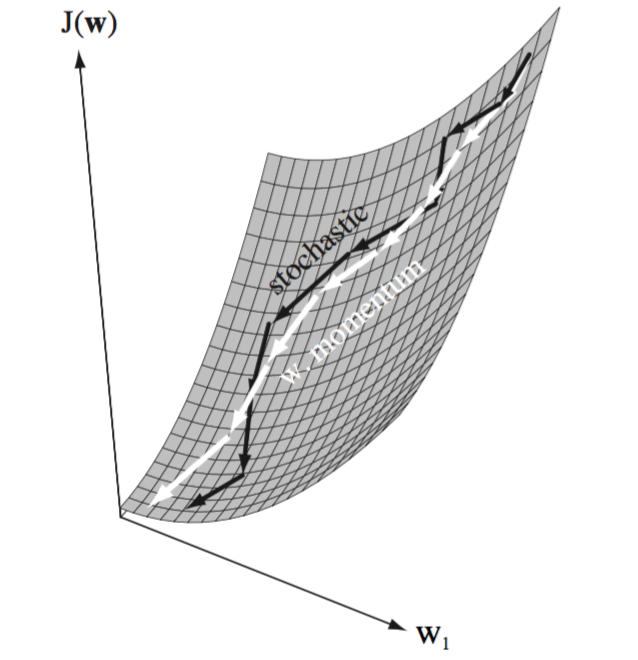
\includegraphics[width=0.8\linewidth]{pic/Momentum}
\end{figure}
Illustration taken from \cite{Duda}
\end{columns}
\end{frame}


%------------------------------------------------
% Section
%------------------------------------------------

\subsection{Nesterov Accelerated Gradient}

\begin{frame}{Nesterov Accelerated Gradient}
\begin{block}{Description}

Like momentum, Nesterov Accelerated Gradient is a first-order optimization method with better convergence rate guarantee. \\~\\

As we have seen with Momentum, adding momentum to the parameter optimization procedure gives us a way to achieve faster convergences, but by momentum, we are adding velocity, we might as well give it a way to "slow down" when it reaches other ramp up.
\end{block}

\end{frame}

\begin{frame}
\frametitle{Nesterov Accelerated Gradient Examples}
\begin{columns}[c] % The "c" option specifies centered vertical alignment while the "t" option is used for top vertical alignment

\column{.9\textwidth} % Right column and width
\begin{figure}
  \caption{Top is a classical momentum trajectory. Down is Nesterov Accelerated Gradient. }
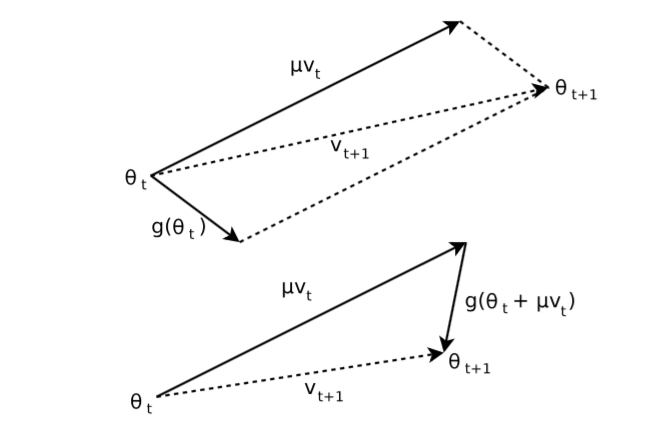
\includegraphics[width=0.8\linewidth]{pic/nesterov}
\end{figure}
Illustration taken from \cite{Hinton}
\end{columns}
\end{frame}

%------------------------------------------------
% Section
%------------------------------------------------

\section{Automated Learning Rate Selection}

\subsection{Introduction}

\begin{frame}{Introduction}
\begin{block}{Description}
Up until now, all method had to be given an explicit learning rate. \\~\\

We remind that this one can be calculated through second order method but that those methods are not always practicable - and even most of the time, unpracticable - thus they don't figure in this list. 
\end{block}

\end{frame}


\subsection{AdaGrad}

\begin{frame}{AdaGrad}
\begin{block}{Description}

Adagrad provides a way to only update parameters that are relevants for a given training example.\\~\\

Doing so, Adagrad provides a way to achieve better robustness. But more : it also remove the needs to tune the learning rate manually
\end{block}

\end{frame}


\subsection{AdaDelta}

\begin{frame}{AdaDelta}
\begin{block}{Description}

Adagrad that seeks to reduce its aggressive, monotonically decreasing learning rate. Instead of accumulating all past squared gradients, Adadelta restricts the window of accumulated past gradients to some fixed size w.
\\~\\
\end{block}
\end{frame}


\subsection{RMSprop}

\begin{frame}{RMSprop}
\begin{block}{Description}

RMSprop comes with the same intuition as AdaGrad. They in fact, have both been developed independently to solve the same issue.

It divides the learning rate by an exponentially decaying average of squared gradients.

\end{block}

\end{frame}


\subsection{Adam}

\begin{frame}{Adam}
\begin{block}{Description}

Adam stands for Adaptifve Moment Estimation

Like AdaGrad and RMSprop Adam also keeps an exponentially decaying average of past gradient

\end{block}

\end{frame}


%------------------------------------------------
% Section
%------------------------------------------------

\section{Annex}

\begin{frame}
\frametitle{Gradient Descent Formalization}

\begin{block}{Basic Gradient Descent Algorithm}
%%%%%%%%%%%%%% PSEUDO CODE GRADIENT DESCENT %%%%%%%%%%%%%%
\begin{algorithmic}
%%% INITIALIZING VARIABLES
\Require $ a, \theta, \eta(.), criterion$

\State $ k \gets 0$
\Repeat
	\State $a \gets a - \eta(k) \nabla J(\theta) $
\Until  $\eta(k) \nabla J(\theta) < criterion$

\Ensure $a$
\end{algorithmic}

\end{block}
\end{frame}


%------------------------------------------------
% Section
%------------------------------------------------

\begin{comment}


\subsection{Subsection Example} % A subsection can be created just before a set of slides with a common theme to further break down your presentation into chunks

\begin{frame}
\frametitle{Paragraphs of Text}
Sed iaculis dapibus gravida. Morbi sed tortor erat, nec interdum arcu. Sed id lorem lectus. Quisque viverra augue id sem ornare non aliquam nibh tristique. Aenean in ligula nisl. Nulla sed tellus ipsum. Donec vestibulum ligula non lorem vulputate fermentum accumsan neque mollis.\\~\\

Sed diam enim, sagittis nec condimentum sit amet, ullamcorper sit amet libero. Aliquam vel dui orci, a porta odio. Nullam id suscipit ipsum. Aenean lobortis commodo sem, ut commodo leo gravida vitae. Pellentesque vehicula ante iaculis arcu pretium rutrum eget sit amet purus. Integer ornare nulla quis neque ultrices lobortis. Vestibulum ultrices tincidunt libero, quis commodo erat ullamcorper id.
\end{frame}

%------------------------------------------------

\begin{frame}
\frametitle{Bullet Points}
\begin{itemize}
\item Lorem ipsum dolor sit amet, consectetur adipiscing elit
\item Aliquam blandit faucibus nisi, sit amet dapibus enim tempus eu
\item Nulla commodo, erat quis gravida posuere, elit lacus lobortis est, quis porttitor odio mauris at libero
\item Nam cursus est eget velit posuere pellentesque
\item Vestibulum faucibus velit a augue condimentum quis convallis nulla gravida
\end{itemize}
\end{frame}

%------------------------------------------------

\begin{frame}
\frametitle{Blocks of Highlighted Text}
\begin{block}{Block 1}
Lorem ipsum dolor sit amet, consectetur adipiscing elit. Integer lectus nisl, ultricies in feugiat rutrum, porttitor sit amet augue. Aliquam ut tortor mauris. Sed volutpat ante purus, quis accumsan dolor.
\end{block}

\begin{block}{Block 2}
Pellentesque sed tellus purus. Class aptent taciti sociosqu ad litora torquent per conubia nostra, per inceptos himenaeos. Vestibulum quis magna at risus dictum tempor eu vitae velit.
\end{block}

\begin{block}{Block 3}
Suspendisse tincidunt sagittis gravida. Curabitur condimentum, enim sed venenatis rutrum, ipsum neque consectetur orci, sed blandit justo nisi ac lacus.
\end{block}
\end{frame}

%------------------------------------------------

\begin{frame}
\frametitle{Multiple Columns}
\begin{columns}[c] % The "c" option specifies centered vertical alignment while the "t" option is used for top vertical alignment

\column{.45\textwidth} % Left column and width
\textbf{Heading}
\begin{enumerate}
\item Statement
\item Explanation
\item Example
\end{enumerate}

\column{.5\textwidth} % Right column and width
Lorem ipsum dolor sit amet, consectetur adipiscing elit. Integer lectus nisl, ultricies in feugiat rutrum, porttitor sit amet augue. Aliquam ut tortor mauris. Sed volutpat ante purus, quis accumsan dolor.

\end{columns}
\end{frame}

%------------------------------------------------
\section{Bibliography Section}
%------------------------------------------------

%------------------------------------------------ %% THE BIBLIOGRAPHIE SECTION

\begin{frame}
\frametitle{References}
\footnotesize{
\begin{thebibliography}{99} % Beamer does not support BibTeX so references must be inserted manually as below

%%%%%%%%%%  Examples %%%%%%%%%
\bibitem{Wind}Model Selection in Data Analysis Competitions 
\bibitem{Duda}Pattern Classification, 2nd Ed (2001), Richard O. Duda , Peter E. Hart , David G. Stork
%\bibitem{Hinton} On the importance of initialization and momentum in deep learning

\end{thebibliography}
}
\end{frame}
%------------------------------------------------


%------------------------------------------------
\section{Second Section}
%------------------------------------------------

\begin{frame}
\frametitle{Table}
\begin{table}
\begin{tabular}{l l l}
\toprule
\textbf{Treatments} & \textbf{Response 1} & \textbf{Response 2}\\
\midrule
Treatment 1 & 0.0003262 & 0.562 \\
Treatment 2 & 0.0015681 & 0.910 \\
Treatment 3 & 0.0009271 & 0.296 \\
\bottomrule
\end{tabular}
\caption{Table caption}
\end{table}
\end{frame}

%------------------------------------------------

\begin{frame}
\frametitle{Theorem}
\begin{theorem}[Mass--energy equivalence]
$E = mc^2$
\end{theorem}
\end{frame}

%------------------------------------------------

\begin{frame}[fragile] % Need to use the fragile option when verbatim is used in the slide
\frametitle{Verbatim}
\begin{example}[Theorem Slide Code]
\begin{verbatim}
\begin{frame}
\frametitle{Theorem}
\begin{theorem}[Mass--energy equivalence]
$E = mc^2$
\end{theorem}
\end{frame}\end{verbatim}
\end{example}
\end{frame}

%------------------------------------------------

\begin{frame}
\frametitle{Figure}
Uncomment the code on this slide to include your own image from the same directory as the template .TeX file.
%\begin{figure}
%\includegraphics[width=0.8\linewidth]{test}
%\end{figure}
\end{frame}

%------------------------------------------------

\begin{frame}[fragile] % Need to use the fragile option when verbatim is used in the slide
\frametitle{Citation}
An example of the \verb|\cite| command to cite within the presentation:\\~

This statement requires citation \cite{p1}.
\end{frame}

%------------------------------------------------

\begin{frame}
\frametitle{References}
\footnotesize{
\begin{thebibliography}{99} % Beamer does not support BibTeX so references must be inserted manually as below
\bibitem[Smith, 2012]{p1} John Smith (2012)
\newblock Title of the publication
\newblock \emph{Journal Name} 12(3), 45 -- 678.
\end{thebibliography}
}
\end{frame}

%------------------------------------------------

\begin{frame}
\Huge{\centerline{The End}}
\end{frame}

%----------------------------------------------------------------------------------------

\end{comment}

\end{document}